\documentclass[aps,prx,reprint,superscriptaddress, longbibliography]{revtex4-1}
\usepackage{H1}
\usepackage[pdftex,colorlinks=true]{hyperref}
\hypersetup{citecolor = blue, linktocpage=true}
\usepackage[normalem]{ulem}
\usepackage{color}
\usepackage[usenames,dvipsnames,svgnames,table]{xcolor}
\usepackage{mathtools}
\usepackage{enumerate}

\usepackage{tikz}
\usetikzlibrary{arrows}

\newcommand{\vedika}[1]{ {\color{red} {{#1}}}}
\newcommand{\david}[1]{ {\color{blue} {{#1}}}}
\newcommand{\charlie}[1]{{\color{Magenta}{{#1}}}}

\newcommand{\Tr}{ \mbox{Tr}}
\renewcommand{\Re}{ \mbox{Re}}
\newcommand{\vb}{v_B}
\newcommand{\I}{\mathbb{I}}
\newcommand{\ip}{i+1}
\newcommand{\mc}[1]{ { \mathcal {{#1}}}}
\newcommand{\Sz}{S_z^{\rm tot}}
\newcommand{\lamv}{\lambda(v)}
\newcommand{\otoc}{{C}({\bf x},t)}
\newcommand{\half}{\frac{1}{2}}
\renewcommand{\ket}[1]{\left|#1\right\rangle}

\begin{document}
\title{Asymmetric butterfly velocities in Hamiltonian and circuit models}
%
\author{Charles Stahl}
\affiliation{\mbox{Department of Physics, Princeton University, Princeton, NJ 08544, USA}}
\affiliation{\mbox{Department of Applied Mathematics and Theoretical Physics, University of Cambridge, Cambridge, UK}}
\author{Vedika Khemani}
\affiliation{\mbox{Department of Physics, Harvard University, Cambridge, MA 02138, USA}}
\author{David A. Huse}
\affiliation{\mbox{Department of Physics, Princeton University, Princeton, NJ 08544, USA}}

\begin{abstract}
	The butterfly velocity $v_B$ has been proposed as a characteristic velocity for information propagation in local systems. It can be measured by the ballistic spreading of local operators in time (or, equivalently, by out-of-time-ordered commutators). In general, this velocity can depend on the direction of spreading and, indeed, the asymmetry between different directions can be made arbitrarily large using arbitrarily deep quantum circuits. Nevertheless, in all examples of local time-independent Hamiltonians that have been examined thus far, this velocity is independent of the direction of information propagation. In this work, we present two models with asymmetric $v_B$. The first is a time-independent Hamiltonian in one dimension with local, 3-site interactions. The second is a class of local quantum circuits, which we call $n$-staircases, where $n$ serves as a tunable parameter interpolating from $n=1$ with symmetric spreading to $n=\infty$ with completely chiral information progagation.  
\end{abstract}

\maketitle

\section{Introduction}
Understanding the dynamics of isolated quantum systems is a topic of fundamental interest. One central question is how isolated systems undergoing unitary time evolution are able to bring themselves to local thermal equilibrium under their own dynamics. Indeed, while all quantum information is always preserved under unitary evolution, it can get ``scrambled" in highly non-local, experimentally inaccessible degrees of freedom - leading to an effective decoherence that can bring local subsystems to thermal equilibrum. 

A useful window into the scrambling process comes from studying the spreading of initially local perturbations under time evolution. Under Heisenberg evolution, a local operator $O_0$ evolves into $O_0(t) = U^\dagger(t) O_0 U(t)$ with support on a spatial region that grows with time. This spreading of quantum information can be diagnosed by the out-of-time ordered commutator (OTOC) which has recently been studied in a variety of systems ranging from strongly quantum chaotic to integrable. The OTOC is defined as $C(\vec{x},t) = \frac{1}{2} \langle [W_\vec{x}, O_0(t)]^\dagger [W_\vec{x}, O_0]\rangle$, where $W_\vec{x}$, $O_0$ are local norm-one operators near positions $\vec{x}$ and $0$ and the expectation value is taken in an appropriate equilibrium ensemble. If $\vec{x}$ is away from the origin, then $W_\vec{x}$ initially commutes with $O_0$ and the OTOC is zero. As the operator spreads, the OTOC grows to become of order one inside a ``light-cone" bounded in all directions by a propagating front. We focus here on chaotic systems with ballistic information spreading at a ``butterfly speed" $v_B(\hat{\vec{n}})$ which may, in principle, depend on the direction of propagation $\hat{\vec{n}}$. The OTOC is related to the commutator norm that appears in Lieb Robinson bounds for local quantum systems, and the Lieb Robinson velocity $v_{LR}$ serves as an upper limit on $v_B$. 

\begin{figure}
	\includegraphics[width=\columnwidth]{LaTeX/circuits.pdf}
	\caption{Random unitary circuits in one dimension. Each gate (rectangular box) is a unitary operator that acts on two adjacent sites and is drawn randomly from some ensemble, such as the uniform Haar measure. The different colors of gates represent different randomly drawn gates. The gates in circuit (a) are random in space and time, while the circuits in (b)-(d) are Floquet circuits which are periodic in time. The ``depth" of the Floquet circuits is set by the time-period which is, respectively, two (b), three (c) and $L$ (d) for a chain of length $L$. The Floquet circuit geometries in (c), (d) are chosen to give asymmetric speeds for information transfer to the left and right, with (d) being a completely unidirectional chiral circuit. 
	}
	\label{fig:circuits}
\end{figure}

Recently, a great deal of insight into the dynamics of operator spreading and quantum entanglement in chaotic systems has been gained by studying various minimally structured coarse-grained models whose time evolution is generated by random unitary circuits. 
Such models are analytically tractable, by design, and are constrained only by locality, unitarity and a few local conservation laws. 
A central assumption, borne out by these studies, is that the time evolution in chaotic systems looks essentially random, so that these ingredients are sufficient for capturing several universal features of the dynamics of thermalizing systems. Several variations have been studied, including unitary circuits that are either random or periodic in time, the latter being the so-called Floquet circuits, and circuits with local unitary gates drawn randomly from various ensembles: for example, uniformly from the Haar measure, or randomly from the Clifford group, or uniformly from the Haar measure subject to various local conservation laws. Figure~\ref{fig:circuits} depicts some of these cases. In addition, one can also consider circuits with random spatial architectures, so that random unitary gates are dropped at random spatial locations at every time step.    

Models of unitary circuits with spatially asymmetric information propagation are straightforward to realize. These include the so-called ``glider" Clifford circuits and the translation operator in one dimension where information propagation is completely unidirectional. The circuit architectures of these models is similar to Fig.~\ref{fig:circuits}(d) where, in the periodic Floquet setting, unidirectional or chiral information propagation requires circuits of infinite depth (time period) scaling with system size $~L$~\footnote{It is possible to get chiral information transport on the edge of a two-dimensional model using only a finite-depth Floquet circuit.}. On the other hand, a finite but unequal ratio of left and right propagation speeds can be achieved using Floquet circuits of finite depth; this is clear from Fig~\ref{fig:circuits}(c) which depicts a period three Floquet circuit built from length three ``staircases" in which operators spread to the right twice as fast as they spread to the left, on average. 
% \charlie{How asymmetric can a circuit of given depth be?}

These examples suggest that asymmetric information propagation can be realized quite generally, and \emph{a priori}, should be realizable even in local, time-independent Hamiltonian systems. Nevertheless, to the best of our knowledge, all examples of local time-independent Hamiltonians that have been examined thus far show symmetric propagation. One of our main results is to construct a time-independent Hamiltonian with local three-site interactions which displays asymmetric information propagation in the left and right directions (Section~\ref{sec:ham}). We quantify the asymmetry by measuring the left and right butterfly speeds, $v_{B, l}$ and  $v_{B,r}$, using various measures of operator spreading. 
Our construction is inspired by results from asymmetric circuit models, and can be easily generalized to realize greater degrees of asymmetry by making the Hamiltonian more non-local. In addition, in Section~\ref{sec:circ}, we also introduce and analyze a class of random circuit models,  called $n$-staircase circuits, in which the asymmetry in butterfly speeds can be tuned by tuning $n$. In such circuits, the ``entanglement generation function" governing the entanglement and operator dynamics, introduced in Ref.~\cite{Cheryne}, can be tuned to have any shape (consistent with the convexity conditions discussed in \cite{Cheryne}). 

\begin{figure}
	\includegraphics[width=\columnwidth]{colorplot}
	\caption{Evolution of the OTOC $C(i,t)$ for an operator initially located at the center of the chain for the model in Equation~\ref{eq:Hammodel}. Data is averaged over 100 disorder samples at $L=15, h=0.35$ with the initial operator at the central site. The bars indicate the time at which the OTOC passes 0.4, to emphasize the asymmetry.}
	\label{fig:colorplot}
\end{figure}

%\tableofcontents

\section{Local Time-Indepedent Hamiltonians with Asymmetric butterfly speeds}
\label{sec:ham}
In this section, we will construct an explicit example of a time-independent local Hamiltonian with asymmetric information propagation. We will work with spin $1/2$ models on a one dimensional lattice with $L$ sites and open boundary conditions, and consider spatially local Hamiltonians of finite range $n$:
\begin{align}
H = \sum_{i=1}^{L-n+1}H_n^{(i)},
\label{eqn:chain}
\end{align}
where $H_n^{(i)}$ is an $n$-site Hamiltonian acting on sites $i$ through $i+n-1$. The degree of asymmetry between the left and right butterfly speeds can by varied by varying $n$. 

Our strategy will be to construct the ``building blocks" $H_n^{(i)}$ to \emph{individually} show some asymmetry in information transfer. Note that $n=2$ will not suffice for this purpose, because 2-site Hamiltonians are always symmetric with respect to their operator dynamics. Unitarity preserves the total amount of information, so if the 2-site Hamiltonian moves some weight from the first site to the second, it must move an equal amount from the second to the first. On the other hand, 3-site Hamiltonians do not have this constraint, and can have asymmetric dynamics. Thus, our minimal example of a Hamiltonian showing asymmetric dynamics will have three-site interactions. 

Instead of looking directly for an asymmetric $H_3$, we can find a unitary operator $U_3$ with the desired dynamics. We can then invert that to obtain $H_3$ such that $U_3=e^{-iH_3}$. One such asymmetric unitary operator is the 3-site cyclic permutation operator $S_{123}$, whose action is defined by:
\begin{align}
S_{123}\ket{\alpha\beta\gamma} =\ket{\gamma\alpha\beta}, \label{eqn:condition}
\end{align}
where $\ket{\alpha\beta\gamma}$ is a product state with state $\ket{\alpha}$ on site 1, etc. Note that this operator can transport a state from site 3 to site 1 in one step, but it takes two applications to move a state from site 1 to site 3. One way to build the three site swap gate is out of 2-site SWAP gates $S_{123} = S_{23}S_{12}$. Each 2-site SWAP interchanges two states, so the action is 
\begin{align}
S_{12}S_{23}\ket{\alpha\beta\gamma} &= S_{12}\ket{\alpha\gamma\beta} = 
\ket{\gamma\alpha\beta}\nonumber\\
&= S_{123}\ket{\alpha\beta\gamma}.
\end{align}
Note that this construction can be easily extended to $n$ sites to create an $n$-site cyclic permutation gate $S_{12\cdots n}$ which can be written as a series of overlapping 2-site SWAP gates. We will come back to this construction in Section~\ref{sec:circ} to build our asymmetric circuits. Indeed, consider a period three Floquet unitary built from the $S_{123}$ gates:
$U = \left(\prod_i S_{123}^{(3i+2)}\right) \left(\prod_i S_{123}^{(3i+1)}\right) \left(\prod_i S_{123}^{(3i)}\right) $
so that the three-site gates at a given time step are non-overlapping in space, but they overlap between time-steps in a three-site generalization of the brickwork circuit shown in Figs~\ref{fig:circuits}(a,b). It is straightforward to show that rewriting the three-site permutation gates as two-site SWAP gates gives a Floquet citcuit whose architecture is equivalent to the asymmetric circuit shown in Fig~\ref{fig:circuits}(c).   

We now invert $S_{123}$ to obtain the desired $H_3$. There are many ways to construct this Hamiltonian, from directly taking the matrix logarithm to analyzing eigenstates. But the simplest way to do this is to note that exchanging any two site indices gives $S_{123}^{-1}$, while overall SU(2) rotations leave the gate unchanged. This means $H_3$ should be antisymmetric with respect to exchanging site indices, and symmetric with respect to SU(2). Therefore $H_3$ is proportional the triple product of the spin on three sites, $H_3 = {\bf S}_1\cdot({\bf S}_{2}\times {\bf S}_{3})$. Putting it together, a candidate Hamiltonian on the full chain is then
\begin{align}
H = \sum_{i=1}^{L-2}{\bf S}_i\cdot({\bf S}_{i+1}\times {\bf S}_{i+2}),
\label{eq:Hamtriple}
\end{align}
where $\bf{S}_i$ are spin 1/2 operators on site $i$. 

In the following subsections, we will numerically analyse the dynamics in the model \eqref{eq:Hamtriple} in more detail, confirming our expectation that this model shows asymmetric operator spreading. In particular, because states and operators evolve in opposite directions, we expect the butterfly velocity in the right direction to be larger for \eqref{eq:Hamtriple}. We also note that the use of 3-site terms has some further consequences. For example, first order perturbation theory will connect site 1 to sites 2 and 3, while second order perturbations connect site 1 to sites 4 and 5. At early time sites 2 will behave the same as site 3, etc., leading to even-odd effects in the spreading. We will correct for this by only looking at alternate sites for each analysis. 

\subsection{Spectral Degeneracies, and Choice of Model}

\begin{figure}
	\includegraphics[width=\columnwidth]{levelrepultrans}
	\caption{Phase transition for the model \eqref{eq:Hammodel}, with the level repulsion parameter $ r$  plotted against the strength of randomness $h$. For small $h$, the r-ratio $ r  \sim 0.6$, appropriate to a chaotic system with GUE statistics, while for large $h$, the r-ratio flows towards the Poisson value of $0.386$ with increasing $L$, characteristic of localization.}
	\label{fig:levelrepultrans}
\end{figure}

While we have confirmed that \eqref{eq:Hamtriple} shows asymmetric operator spreading, the dynamics in this model suffers from various non-generic peculiarities due to the presence of several additional symmetries, with one symptom being an exponentially large degeneracy of energy eigenvalues at $E=0$. To see this, note that \eqref{eq:Hamtriple} anticommutes with inversion symmetry $\mathcal{I}$ so that the eigenenergies come in $\pm E$ pairs for $E\neq0$. It is straightforward to show that in the presence of operators $R$ such that $\{H, R\}=0$, the degeneracy of the zero-energy manifold is lower-bounded by $\mbox{Tr}(R)$~\cite{IadecolaFSUSY}. The inversion operator $\mathcal{I}$ is one such operator with $\mbox{Tr}(\mathcal{I}) \sim 2^{L/2}$, partially explaining the zero-energy degeneracy. In fact, for even length chains, the degeneracy is even larger than $\mbox{Tr}(\mathcal{I})$ because of the presence of the additional $SU(2)$ symmetry. If we break the $SU(2)$ symmetry down to $U(1)$, say by adding a uniform field in the $Z$ direction, then $\mathcal{I}$ no longer anticommutes with $H$, but $R = P_x \mathcal I $ does, where $P_x = \prod_i S_i^x$. In this case, $\mbox{Tr}(R)$ gives the zero energy degeneracy for both even and odd $L$. Finally, we can get rid of all degeneracies by adding a random field in the $Z$ direction, so that the Hamiltonian is 
\begin{align}
H = \sum_{i=1}^{L-2}{\bf S}_i\cdot({\bf S}_{i+1}\times {\bf S}_{i+2}) + 
\sum_{i=1}^{L}h_iS_i^z,
\label{eq:Hammodel}
\end{align}
where each $h_i$ has a uniform probability distribution on $[-h,h]$. 

While the model above \eqref{eq:Hammodel} certainly gets rid of various peculiarities present in the dynamics of \eqref{eq:Hamtriple}, the random field introduces the possibility of localizing the system for large enough $h$. One widely used diagnistic of localization is the level spacing ratio, defined as $r_n = \rm{min}(\Delta E_{n+1}/\Delta E_n,\Delta E_{n}/\Delta E_{n+1})$ where $\Delta E_n = E_n - E_{n-1}$ and $E_n$ is the $nth$ energy eigenvalues. This parameter is a probe of the level repulsion in the eigenspectrum, and the spectrally averaged $r_n$, $r$, flows towards the GUE value $0.6$, while it flows towards the Poisson value $0.386$ in a localized system. 
In Fig.~\ref{fig:levelrepultrans}, we plot $r$ as a function of $h$ \vedika{averaged over the middle xxx of the spectrum and xxx disorder realizations}, and see a transition to a localized phase near $h \sim 3$. To steer clear of both the $h=0$ and large $h$ limits, we work with $h \sim 0.35$ for the balance of this paper. This field is also small enough that the dynamics are still dominated by the triple-product term, leading to the desired asymmetry (see Fig.~\ref{fig:colorplot}). 


% As we continue to increase $h$ the model moves through the thermalizing phase and becomes localized. In the large-$L$ limit the transition from ergodic to localized is a phase transition, described in~\cite{1010.1992v1}. The transition for the present model can be seen in Fig.~\ref{fig:levelrepultrans}, showing the ratio of adjacent energy gaps. Note that at smaller $L$ the model also drifts away from GUE statistics at very small $h$, when the field is no longer large enough to sufficiently lift the $E=0$ degeneracy. In order to avoid both of these regimes, we will perform all calculations with $h=0.35$. 



\subsection{Asymmetric butterfly speeds from left/right operator weights}

We now turn to an analysis of the asymmetric butterfly speeds in \eqref{eq:Hammodel} measured through the spreading of local operators. For spreading in the right (forward) direction, the initial operator is placed on site 1, while for spreading in the left (backwards direction), the initial operator is placed at site $L$. We will quantify the asymmetry in spreading speeds using two metrics: the right/left weights and the OTOC. 

\begin{figure}
	\includegraphics[width=\columnwidth]{Rweightpeakshape}
	\includegraphics[width=\columnwidth]{Rweighthalftimes}
	\caption{(top) Right weights (solid lines) and left weights (dashed lines) at even distances $x$ from the starting site for $L=13$, $h=0.35$, averaged over 100 disorder realizations. For $\rho_r(1+x,t)$, the initial operator is $\sigma^z_1$ while for $\rho_l(L-x,t)$ the initial operator is $\sigma^z_{L}$. The peaks travel ballistically, and curves for $x=0$ and $x=L-1=12$ are excluded for clarity. The symbols $\times/+$ mark the time at which the right/left weights reach half their maximum peak height for a given distance $x$. The right weight peaks earlier at later times, signifying a faster butterfly velocity in the forward direction.
		(bottom) Time of half-peak for right/left weights vs. distance $x$. The linear fit confirms ballistic propagation of the left and right fronts. Since this is plot of time as a function of distance, the larger slope in the left weight means that $v_B$ is larger for propagation to the right. 
	}
	\label{fig:Rweightpeakshape}
\end{figure}

To define the right and left weights, note that in a spin 1/2 system of length $L$, a complete orthonormal basis for all operators is provided by the $4^L$ ``Pauli strings" $\mathcal{S}$ which are products of distinct Pauli operators $\{1, \sigma^x, \sigma^y, \sigma^z \}$ on each site:
$O(t) = \sum_{\mathcal{S}} a_\mathcal{S}(t) \mathcal{S}$. Unitarity enforces that the norm of the operator is constant for all times, which means $\sum_{\mathcal{S}} |a_\mathcal{S}(t)|^2 =1$ for a normalized operator. 
An initially local operator, at early times, consists only of strings $\mathcal{S}$ that are the local identity everywhere except near the starting position. But, with time, the operator weight spreads to longer Pauli strings, containing
non-identity local operators at sites out to fronts whose distance from the origin grows ballistically with time. It is this operator growth that we will be measuring in both the right and left directions. On useful diagnostic of this is provided by the right (left) weight of the operator, which is the total weight of $O(t)$ on Pauli strings that have their rightmost (leftmost) non-identity operator on site $i$, and act as the local identity on all sites to the right (left) of $i$:
\begin{align}
\rho_r(i,t)= \sum_{\substack{{\text{strings $\mc{S}$ with } }\\ \mathclap{\text{ rightmost non-}}\\ \mathclap{\text{identity on site $i$}}}} |a_\mc{S}(t)|^2.
\end{align}
The left weight $\rho_l(i,t)$ is defined analogously.  If $ O$ is initially local on site $j$ then $\rho_r(i,0) = \rho_l(i,0) = \delta_{ij}$. The conservation of operator norm implies that $\sum_i \rho_{r/l}(i,t)=1$, which gives $\rho$ the interpretation of an emergent local conserved `density" for the right/left fronts of the spreading operator. Refs.\cite{opspreadAdam, opspreadCurt} showed that the (hydro)dynamics for $\rho_R(i,t)$ is governed by a biased diffusion equation, corresponding to fronts that propagate ballistically but broaden diffusively. Thus, as the operator spreads, $\rho_r$ moves right at $v_{B,r}$ and $\rho_l$ moves left at $v_{B,l}$. 

In order to compare the propagation of the left- and right fronts, we look at  $\rho_r(x_r+1,t)$ and $\rho_l(L-x_l,t)$. Thus, $x_{r}$ and $x_l$ are distances from the initial operator located at the left/right ends respectively. Note that $i$ runs from 1 to $L-1$ because it is a label while $x$ runs from 0 to $L$ because it is a distance. Fig.~\ref{fig:Rweightpeakshape}(top) shows $\rho_r(x_r+1,t)$ and $\rho_l(L-x_l,t)$ at successive times for different spatial separations $x_{l/r}$ from the starting locations in a system of size $L=13$, clearly showing ballistically traveling operator fronts. Note that the weights at equivalent distances from the ends of the chain peak at later times for the left-moving wave,  clearly showing $v_{B,l}<v_{B,r}$. More quantitatively, we can extract $v_{B,l}$ and $v_{B,r}$ from these curves by obtaining the times at which $\rho_{r/l}$ reach half their maximum peak height for a given distance $x$ (denoted by crosses/pluses on Figure~\ref{fig:Rweightpeakshape},top), and fitting these to linear functions (Figure~\ref{fig:Rweightpeakshape}, bottom). This procedure gives $v_{B,r}=1.011 \pm 0.072$ and $v_{B,l}=0.791 \pm 0.062$, showing a clear asymmetry in the butterfly speeds in the two directions. 

As mentioned earlier, because of the nature of the three-site term in the Hamiltonian, the right/left weights exhibit an ``odd-even" effect where site 3 may peaks before 2, etc (also visible in Fig.~\ref{fig:colorplot}). It is possible to account for these by averaging judiciously, or by  looking at only alternate sites, which is why we only show even distances in Figure~\ref{fig:Rweightpeakshape}. 



\subsection{Asymmetric butterfly speeds from OTOCs}

We now turn to a complementary measure of operator spreading, namely the out-of-time-ordered commutator $C(i,t)$, defined for $\sigma^z$ operators as: 
\begin{align}
C(i,t) & = \half \langle|[\sigma^z_j(t),\sigma^z_i(0)]|^2\rangle_{\beta=0}\nonumber\\
&= 1 - \frac{1}{2^{L}}\Re\;\Tr\;[\sigma^z_j(t)\sigma^z_i(0)\sigma^z_j(t)\sigma^z_i(0)]
\label{eq:otoc}
\end{align}
where $j$ is the site index of the initial operator, and the expectation value in the top row is with respect to a thermal ensemble at infinite temperature. As discussed earlier, the OTOC is of order one inside a ballistically growing light-cone defined by the left and right butterfly speeds, and exponentially small outside it.  Fig.~\ref{fig:colorplot} shows the OTOC for an operator initially at the center of the chain, and the lightcone is approximately demarcated by where $C(i,t)= .4$, illustrated by the black bars. The figure again visually shows $v_{B,r} > v_{B,l}$.  The light-cone in the figure is not strictly monotonic because of the even-odd effects mentioned earlier. 


\begin{figure}
	\includegraphics[width=\columnwidth]{oddVDLEfromOTOCs}
	\includegraphics[width=\columnwidth]{oddVDLE}
	\caption{Velocity-dependent Lyapunov exponents extracted from the OTOC on odd sites. The parameters are $L=15, h=0.35$, while the OTOC is as defined in the text with initial operators at sites 1 and $L-1$ respectively. Statistics are obtained from 100 disorder realizations. The top figure shows the early-time right-moving OTOCs on a semilog plot. VDLEs are obtained from the best fit line through odd sites. The lower figure shows $\lambda(v)$. Since $\lambda_r(v)>\lambda_l(v)$, we know $v_{B,r}>v_{B,l}$.}
	\label{fig:vdle}
\end{figure}

The OTOC $C(i,t)$ is widely regarded as a diagnostic of chaos because, in many systems of interest, it shows an exponential increase from a value near zero to an order one number as the site $i$ enters the light-cone of the spreading operator, $C(i,t) \sim \epsilon e^{\lambda t}$ where $\lambda >0$ is a positive Lyapunov exponent. This is closely related to the exponential sensitivity of classically chaotic systems to small perturbations in initial conditions. However, an important point is that in quantum systems this exponential growth only takes place in systems which are in certain semiclassical or weakly coupled or large $N$ limits, and not in ``strongly-quantum" systems away from such limits --- such as strongly interacting thermalizing spin 1/2 chains which are the subject of this paper. Thus, no well-defined positive Lyapunov exponent exists in such strongly quantum systems. Nevertheless, Ref.~\cite{Khemani2018lambda} showed that one can still define \emph{velocity dependent} Lyapunov exponents (VDLEs) in these cases,  and these can be used to provide a more detailed window into asymmetries in information propagation 



As in the case of the right-weight case, we set $j=1$ to measure $v_{B,r}$ and $j=L-1$ to measure $v_{B,l}$. The OTOC should be order-1 inside the lightcone and exponentially small outside the lightcone defined by $v_B$. 




\charlie{Move this paragraph to an appendix?}
From conservation of $\Sz$, the Hamiltonian and all relevant operators are block-diagonal, with the size of the $i^\text{th}$ block being $\binom{L}{i}$. For smaller blocks we can compute the trace directly, but for larger blocks this becomes computationally difficult. We then rely on quantum typicality to approximate the trace in the large blocks. For each disorder realization we replace the trace with an average over expectation values in pure states~\cite{Luitz2017}. The pure states are chosen Haar-randomly, and we find that using 5 vectors gives relative errors around 0.05 for blocks larger than $500\times 500$. For smaller blocks we use exact diagonalization.

The VDLEs quantify how fast signals decay along constant-velocity trajectories outside the lightcone. In particular, if the OTOC is measured along the ray defined by each site $i$ at time $t_i = i/v$ for some $v$, then it should decay exponentially,
\begin{align}
C(i, t) \sim e^{\lambda(v)t}\quad\text{for}\quad i = vt.
\end{align}
Ref.~\cite{Khemani2018lambda} gives a thorough exposition and explanation of VDLEs. The name comes from the fact that the Lyapunov exponent defines how fast a signal grows inside a lightcone in a classically chaotic system. 

In the current system, the OTOCs are influenced by the previously-mentioned odd-even effects. We can once again look only at odd sites for sufficiently large $L$ to calculate $\lambda(v)$. Then $v_B$ is the velocity at which $\lambda(v)$ smoothly goes to 0. If we again look at Fig.~\ref{fig:colorplot}, $v_B$ will be the ray that passes through the black bars. Hence, we can already see the asymmetry before calculating $v_B$ explicitly. 

Fig.~\ref{fig:vdle} illustrates the process of finding $\lambda(v)$ and shows the VDLEs for the right-going and left-going OTOCs, estimated from the odd sites. Note that in the top plot the independent variable is distance, so the slope of the best fit line is $\lambda(v)/v$.
Finite-size effects slightly perturb $\lambda(v)$ around $v_B$, but we can see that $v_{B,l} \sim 0.5$ and $v_{B,r} \sim 0.9$. Analysis of the odd sites is less clean, but suggests $v_{B,l} \sim 0.5$ and $v_{B,r} \sim 0.7$.
These are not very close to the velocities estimated from the right weight. Since $v_B$ is \charlie{well defined} only in the thermodynamic limit, we expect these methods to agree as $L\to\infty$.



\section{Circuit models} \label{sec:circ}

We will now discuss a different system that also displays asymmetric spreading and can be completely chiral in a certain limit. Instead of a time-independent Hamiltonian, this system is a random quantum circuit. Random unitary circuits are discussed in .... The setting for the system is again a spin chain of length $L$, but we allow the dimensionality of each site to be $q\ge2$. Eventually we will take the limit $q\to\infty$. At discrete times, unitary operators called gates act on pairs of consecutive sites. We will refer to the spaces between sites as bonds, so that each pair of sites is specified by a bond index. In contrast to the previous section we will refer to the sites with index $i$ and bonds with index $x$.

Our random circuit will have two sources of randomness. The first will be in the choice of gates, which will be independently chosen from the Haar distribution, which assigns an equal probability to any gate in the space of unitary two-site operators. The second will be in our architecture. A purely random architecture would have a bond chosen at random at each time step. We consider a generalization of this architecture, which we call the staircase architecture, described by the staircase size $n$. The staircase circuit consists of $n$-stairs at random bonds. 
Each $n$-stair is defined by always having strings of $n$ gates act on bonds $x$ through $x+n-1$ in succession. For $n=1$ this is just a random architecture, but large $n$ results in more asymmetric circuits. For $n=L$, the circuit would always have a gate at bond $x+1$ after bond $x$.

We will be interested in circuits with infinite $L$. When $n$ is small we can extract the behavior from systems with finite $L>>n$. For large $n$ we can first take $L\to\infty$ and then $n\to\infty$ or set $n=L$ and take them to $\infty$ together. The behavior does not depend on the order of limits, but it is easier to reason about the circuits using the second procedure.

The structure of this section is as follows. Sec.~\ref{sub:entropy} describes how the butterfly velocity for random unitary circuits can be extracted from the entropy growth rate. In Sec.~\ref{sub:classical} we show that the limit $q\to\infty$ results in classical dynamics for the entropy. Finally in Sec.~\ref{sub:asym} we explore $v_B$ for these circuits. The transport is symmetric for $n=1$ (random circuit) and completely asymmetric for $n=\infty$. Although the model is not solvable for intermediate $n$, we provide an approximation to the entropy growth function that is correct at $n=1, \infty$.

\subsection{Entropy in random circuits} \label{sub:entropy}

%Before discussing asymmetric circuits we will explain how $v_B$ can be extracted from the growth of entanglement. We will then show that this method is particularly tractable in the large-$q$ limit before applying this method to staircase circuits. 
%Consider a spin chain of $L$ sites, each with dimension $q$. Sites are labeled by $i = 1,\dots, L$ , while the bonds between sites are labeled by $x = 1, \dots, L - 1$. 

Define the entropy function $S(x)$ as the bipartite entanglement entropy across bond $x$. 
After course-graining, the entanglement becomes a continuous function $S(x,t)$. Given a circuit architecture, the entanglement growth rate is to first order only a function of the slope, so we can write \cite{Jonay}
\begin{align}
\frac{\partial S}{\partial t} = \Gamma\left(\frac{\partial S}{\partial x}\right).
\end{align}
It is useful to define the entropy density $s = \partial S / \partial x$, which is so-called because the equilibrium entropy is $S(x, t) = s_\text{eq} \min\{x, L - x\}$.  In the next subsection we will show that the maximal slope is 1. In general the equilibrium slope can be smaller than 1, but since our systems are noisy, $s_\text{eq} = s_\text{max} = 1$.

This function $\Gamma(s)$ encodes the butterfly velocity as the derivative $\Gamma'(s)|_{s_\text{ext}}$, where $s_\text{ext}$ is one of the extremal entropy densities, 1 or $-1$. 
\begin{align}
v_{B,l}=\left.\frac{\partial \Gamma}{\partial s}\right|_{s=-1}, 
v_{B,l}=\left.\frac{\partial \Gamma}{\partial s}\right|_{s=-1} 
\label{eqn:vbGamma}
\end{align}
A brief explanation of why this is the case is given in the appendix, while a stronger argument can be found in Ref.~\cite{Jonay}
It follows that any $\Gamma(s)$ with asymmetry at the endpoints will have asymmetric butterfly velocities.

\subsection{Classical dynamics of $q\to\infty$ limit} \label{sub:classical}

We will consider entropy functions $S(x,t)$ defined on a periodic system of length $L$. The boundary conditions are $S(x+L,t) = S(x,t)+sL$, allowing for an overall entanglement density $s$. We will only consider linear entropy functions, so the use of $s$ as a local and global entropy density does not conflict.
Subadditivity tells us ${|S(x + 1)-S(x)|} \le S_1$, where $S_1$ is the entropy at a single site. If we take our logarithms with base $q$, then $S_1 \le 1$. After coarse-graining this gives the result $s_\text{ext}=\pm1$.

If a gate acts on bond $x$, it can increase the bipartite entanglement entropy $S(x)$, up to the constraint $|S(x + 1) - S(x)| \le 1$. In the $q\to\infty$ limit, a Haar-random gate will, with probability 1, maximally increase the entanglement across the bond it acts on~\cite{nahum2017quantum}. Given the previous constraint, this means that if a gate acts at bond $x$ at time $t$, then $S(x, t+1) = \min\left\lbrace S(x-1,t)+1, S(x+1,t)+1\right\rbrace$. \charlie{Should we explain why?} For the remainder of this paper we will use the $q\to\infty$ limit.

At this point, all quantum effects leave the system, and the information dynamics are purely classical. This means it is possible to simulate the circuit without diagonalizing any Hamiltonians or unitary operators. It suffices to consider integer-valued $S(x)$ with $|S(x)-S(x-1)|=1$ for all $x$. Any other state, with either non-integer $S(x)$ or flat steps, will approach one with these characteristics. A state of this form can be described as a series of up and down steps at each site. We will write these as $u$ and $d$. If a gate falls on bond $x$, it adds two units of entropy to $S(x)$ iff the step before is $d$ and the step after is $u$. This classical evolution is deterministic and can be easily simulated.
Since individual circuits have deterministic behavior, we average over circuit architecture (the random placement of $n$-stairs).

Figure \ref{fig:stairs} illustrates the evolution of the entropy function for a single application of a 4-stair. The stair consists of 4 individual gates. Each gate has height 2 because if it produces entropy, it produces 2 units. The shaded profile is the initial $S(x)$, while the dashed line shows $S(x)$ after the $n$-stair falls. The first, second, and fourth gates were productive while the third was not.
\begin{figure}
	\includegraphics[width=\columnwidth]{stairs}
	\caption{A 4-staircase falling on an example entropy function. Note that each gate raises $S(x)$ by 2 iff $S(x)$ is a local minimum when that gate falls. So the second gates does in fact hit a local minimum because it acts after the first gate.}
	\label{fig:stairs}
\end{figure}
It is already possible to see the origin of the asymmetry. The 4-staircase can only be perfectly effective (produce 8 units of entropy) if it hits the microstate ${d,u,u,u}$. Any other state will result in the production of less entropy, if any. Since this microstate has positive slope, it is more likely to be found when the overall slope of the system is larger.

To set a time scale for the system we neet a rate at which gates are applied. The gate rate $\gamma$ is defined as the number of gates per unit time, not staircases. This means that as if every gate is productive, the entropy growth rate is $\Gamma=2\gamma$. The rate at which complete staircases fall is $\gamma/n$.

\subsection{Asymmetric $v_B$} \label{sub:asym}

Despite the deterministic evolution of these circuits, they cannot be solved for finite $n>1$. This is due to correlations that arise in the up and down steps of $S(x)$. If these steps were uncorrelated, then a general state could be described solely by the slope $s$. At any bond the probability of $u$ would be $(1+s)/2$ and the probability of $d$ would be $(1-s)/2$. Correlations make the probability of an $u$ dependent on the surrounding steps. 

There are no correlations in the $n=1$ model, so we can exactly solve the entropy growth function.
Since a gate is productive only at a local minimum, the probability that a randomly placed gate is productive is $(1+s)(1-s)/4$. Then the entropy growth rate is the gate rate, times the probability of entropy production, times the entropy produced per gate:
\begin{align}
\Gamma_1(s)=\gamma\frac{(1+s)(1-s)}{4}2 = \gamma\frac{1-s^2}{2}
\end{align}
For larger $n$ we can perform a similar analysis. Although we know correlations will affect the growth rate, hopefully the effect is small. 


2-stairs consist of one gate acting at bond $x$ and one at bond $x+1$. The entropy production of these gates is affected by the slope between the two bonds and the slopes on either side. There are 8 possible configurations of those three slopes, but only 4 result in entropy growth, as shown in table~\ref{tab:2stair}. Weighting each configuration by its probability and the entropy generated, and then multiplying by the staircase rate $\frac{\gamma}{2}$, the growth rate is approximately
\begin{align}
\Gamma_2(s) 
% &= \frac{\gamma}{2} 4\frac{1+s^2}{4}\frac{1+s}{2} + \frac{\gamma}{2}
% 	2\frac{1-ms2}{4}
% 	\left(\frac{1-s}{2} + \frac{1-s}{2} + \frac{1+s}{2}\right) \nonumber\\
&= \frac{\gamma}{2}\frac{1-s^2}{2}\frac{5+s}{2}, \label{eqn:2rate}
\end{align}
We can interpret the factor $\frac{1-s^2}{2}\frac{5+s}{2}$ as the average entropy produced by each staircase. The second factor provides the asymmetry.

\begin{table}
	\centering
	\begin{tabular}{ccc}
		Initial $\to$ Final 
		Configuration        & Probability         & Productivity\\
		$d\,u\,d\to u\,d\,d$ & $\frac{1-s}{2}\frac{1+s}{2}\frac{1-s}{2}$ & 2\\
		$d\,u\,u\to u\,u\,d$ & $\frac{1-s}{2}\frac{1+s}{2}\frac{1+s}{2}$ & 4\\
		$d\,d\,u\to d\,u\,d$ & $\frac{1-s}{2}\frac{1-s}{2}\frac{1+s}{2}$ & 2\\
		$u\,d\,u\to u\,u\,d$ & $\frac{1+s}{2}\frac{1-s}{2}\frac{1+s}{2}$ & 2
	\end{tabular}
	\caption{The four configurations that result in entropy growth for 2-stairs, the relative proportions of the initial states assuming an uncorrelated entropy distribution, and the growth in entropy generated by a 2-stair falling on that configuration. The four configurations that do not result in entropy growth are $u\,u\,u, d\,d\,d, u\,d\,d,$ and $u\,u\,d$.}
	\label{tab:2stair}
\end{table}

We can determine the growth rate for arbitrary length stairs through a recursive relationship. Consider a staircase made of $n$ gates. Like in the $n=2$ case, its growth rate will be proportional to the staircase rate $\frac{\gamma}{n}$ multiplied by the average entanglement generated by each staircase, so we can write
\begin{align}
\Gamma_n(s) = \frac{\gamma}{n}R_n(s), \label{eqn:growthrate}
\end{align}
where $R_n(s)$ is the average entropy production of an $n$-stair. To find an equation for $R_n(s)$, note that the first $n-1$ gates have the same entanglement production as the $(n-1)$-stair. All final states of the $(n-1)$-stair end in a down slope, so the $n$th gate will produce another 2 units of entropy if the last step is $u$. However, if all $n+1$ initial steps are $u$ no entanglement is generated. 

This behavior is captured by the recursive formula
\begin{align}
R_n(s) = R_{n-1}(s)+2\frac{1+s}{2} - 2\left(\frac{1+s}{2}\right)^{n+1}, \label{eqn:raterecur}
\end{align}
along with the base case $R_0(s)=0$. The solution is
\begin{align}
\Gamma_n(s) = \frac{\gamma}{n}\frac{1+s}{1-s}\bigg(
(1+s)&\left[\left(\frac{1+s}{2}\right)^n-1\right]\nonumber \\
&+n(1-s)\bigg). \label{eqn:growthrate}
\end{align}
Then, from Eqn.~\ref{eqn:vbGamma}, $v_{B,l}=\gamma$ while $v_{B,r}=\half\gamma(n+1)$.
This produces successively more asymmetric butterfly velocities as $n$ increases. 

The question becomes, how much of an effect do the correlations have? 
For small $n$, we can simulate the classical dynamics numerically for finite $L>>n$. This will capture the correct correlation behavior. For the growth rate curves of $n$-stair circuits for $n\le 6$ see Fig.~\ref{fig:compareRates}. 
\begin{figure}
	\includegraphics[width=\columnwidth]{predicRates.pdf}
	\includegraphics[width=\columnwidth]{compareRates.pdf}
	\caption{Predicted and empirical growth rate as a function of slope for $n$-stair circuits. The predicted growth rate consistently overestimates, but captures the general pattern. The right/forward and left/backward butterfly velocities are the slopes of these curves at their endpoint, indicating that as the left $v_B$ stays constant, the right $v_B$ increases. The appendix includes an argument that the right $v_B$ is unbounded in the large-$n$ limit. All growth rates were calculated using a 100-site spin chain with offset periodic boundary conditions. Rates were calculated from the application of 2,000 gates total, or 20 per site, averaged over the last 80\% of the gates in order to build up correlations, then averaged over 100 trials.}
	\label{fig:compareRates}
\end{figure}
The asymmetry is evident for all $n>1$, and the asymmetry continues to increase as $n$ increases. The growth rates follow the same pattern as the predicted rate, although they are smaller overall. 

Simulation becomes difficult as $n$ increases.
Luckily, as $n$ becomes very large (for infinite $L$) or approaches the size of the system (for finite $L$), the correlations again become unimportant. To see this we show that the predicted growth rate is correct at various $s$.
Consider $s = -1, 0,$ and 1 for $n=L$ stairs. At exactly $s=\pm1$ there will be no growth, so we consider an entropy function with a single up or down step before sending $L\to\infty$.

The predicted growth rate is $\Gamma_\infty(s)=\gamma(s+1)$. Near $s=-1$, the entropy profile consists of down steps with a single $u$. Then the circuit generates entanglement once every time a staircase falls. We determine $\Gamma_\infty(-1)=\gamma/L$, which approaches 0 as $L$ becomes large.

In the $m = 0$ case, after a gate falls between sites $i$ and $i + 1$, $s_{i+1}$ will be a down slope regardless of whether the gate generated entanglement. Then the next gate falls across sites $i + 1$ and $i+2$. At site $i+2$ $s_{i+2} = u$ with probability $\half$, so on average $\half$ of the gates produce 2 units of entanglement and $\Gamma_\infty(0)=\gamma$. At near-maximal slope nearly all slopes are $u$, except at the site to the right of the most recent gate. Then the next gate falls at a local minimum with probability 1, and all gates produce 2 units of entanglement, so $\Gamma_\infty(1)=2\gamma$.

Because these rates match the predicated rate, we know it is exact at $s=0, \pm1$. From concavity, the only possible function is then $\Gamma_\infty(s)=\gamma(s+1)$. This shows that our approximation again becomes exact at $n=\infty$ and the system achieves chiral transport. The butterfly velocities are $v_{B,l}=\gamma$ and $v_{B,r}=\infty$. Although we do not know the exact behavior for $1<n<\infty$, we know it interpolates between symmetric and completely asymmetric behavior.

\section{Conclusion}

Asymmetry in $v_B$ is possible, but is limited by locality. In time-independent Hamiltonian systems locality is measured by the range of interactions, while in circuits it is related to the depth. This paper studied both types of systems, showing that local Hamiltonians can support asymmetric spreading and probing spreading in nearly-local circuits. 

The advantages of the Hamiltonian system are that it is a general model. Each site is only a 2-level system. The random field allows the model to be tuned within the thermalizing phase, which could be useful in watching the asymmetry dissipate as the system approaches the phase transition. 

The system studied in this paper is not the only possible 2-nearest-neighbor system. Another interesting direction of research would be how to find maximally asymmetric Hamiltonians for a given interaction length. With more sites per term it would also be possible to study 2-D systems with anisotropic $v_B$.

The class of circuit models studied here provide the opportunity to interpolate between symmetric circuits and completely chiral circuits by varying $n$. One important generalization is to consider finite $q$, the dimension of the Hilbert space at each site. Ref.~\cite{KeyserlingkHydro} suggest that this will lead to a slower $v_B$ as well as $v_E<v_B$. The separate velocity scale $v_E$ leads to operator spreading in individual circuits, not just the ensemble averages this paper discusses.

%We'll want to cite a bunch of people~\cite{Larkinotoc,Lieb72,KitaevSYK,chaosbound,HosurYoshida,ShenkerStanfordButterfly,LocalizedShocks,CotlerRM,RobertsStanford,GuQiStanford,GuQi_rcft,StanfordWeakCoupling,PatelDiffusiveMetal,ChowdhuryON,Galitski_lyapunov,DoraMoessner,LuitzScrambling,ProsenWeakChaos,AleinerOTOC,MotrunichTFIM_otoc,FradkinHuse,ChalkerFloquetChaos,FawziScrambling,opspreadAdam, opspreadCurt, TiborCons, KhemaniCons}.

\section*{Acknowledgements}
We thank many people.

\charlie{Note somewhere about arXiv:1809.02614v1}

\appendix

\section{Butterfly velocity from $\Gamma(s)$}

To see why $\Gamma'(s_\text{ext})$ gives $v_B$, consider a region in which the entropy profile is piecewise linear, with $S'(x<x^*)=s_1$ and $S'(x>x^*)=s_2$. Also note $\Gamma(s)$ is always convex. This is certainly true for the functions considered above, and is also true in general. Then if $s_1<0<s_2$, the transition between the region stays sharp. If it did not, a curve would form with intermediate slopes $s_1<S'(x)<s_2$. But from convexity all of this region would have a faster entanglement growth than $\min\{s_1,s_2\}$ and the peak would reform. 
This peak location $x^*$ travels at velocity $\dot{x}*=-\frac{\Gamma(s_2)-\Gamma(s_1)}{s_2-s_1}$, the slope of the chord connecting $\Gamma(s_2)$ and $\Gamma(s_1)$. See Fig~\ref{fig:entanglevel} for an illustration of this configuration.
\begin{figure}
	\centering
	\begin{tikzpicture}
\draw[->] (-.5,0) -- (5,0) node[below right]{$x$};
\draw[->] (0,-.5) -- (0,4) node[below left]{$S(x,t)$};
\draw[] (0,1) -- (3.5,1) -- (4.5,0);
\draw[->] (1,1.3) -- (1,2.2) ;
\draw (1.5,1.5) node{\small $\Gamma(0)$};
\draw (0,2.5) -- (2,2.5) -- (3.5,2.5);
\draw[dashed] (2,2.5) -- (3.5,1);
\draw[->] (3.2,3) -- (2,3) node[above right]{\small $v_E$};
\draw (4.5,.8) node{\small $m=-1$};
\draw (1.5,.7) node{\small $m=0$};
\end{tikzpicture}
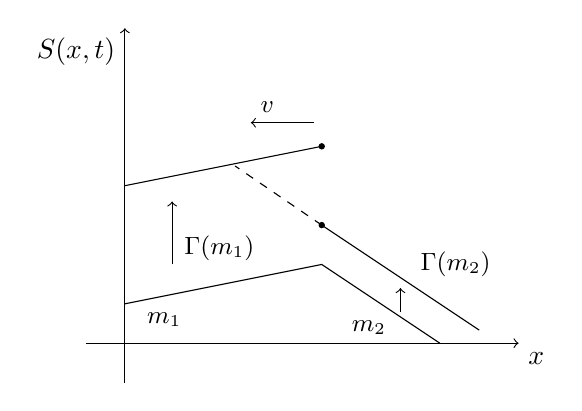
\begin{tikzpicture}
\draw[->] (-.5,0) -- (5,0) node[below right]{$x$};
\draw[->] (0,-.5) -- (0,4) node[below left]{$S(x,t)$};
\draw (0,0.5) -- (2.5,1) -- (4,0);
\draw (0,2) -- (2.5,2.5) node[draw,shape=circle, fill=black, scale=.2]{} (2.5,1.5) node[draw,shape=circle, fill=black, scale=.2]{} -- (4,.5) -- (4.5,.1666);
\draw[->] (.6,1) -- (.6,1.8) ;
\draw[->] (3.5,.4) -- (3.5,.7) ;
\draw (1.2,1.2) node{\small $\Gamma(m_1)$}
      (0.5,0.3) node{\small $m_1$}
      (4.2,1.0) node{\small $\Gamma(m_2)$}
      (3.1,0.2) node{\small $m_2$};
\draw[dashed] (2.5,1.5) -- (1.4,2.25);
\draw[->] (2.4,2.8) -- (1.6,2.8) node[above right]{\small $v$};
\end{tikzpicture}
	\caption{Velocity of a kink between linear section of the entanglement function. Both sections grow at the growth rates defined by their slopes. To maintain continuity the kink moves at $v=-\frac{\Gamma(m_2)-\Gamma(m_1)}{m_2-m_1}$.}
	\label{fig:entanglevel}
\end{figure}

If instead, $s_1>0>s_2$, the kink does not remain sharp. The sharp point $x^*$ becomes a smooth curve, running tangent to the two linear sections at $x^*_l$ and $x^*_r$. By a similar argument to the above, these features travel at $\dot{x}^*_l-\Gamma'(s_{1}), \dot{x}^*_r-\Gamma'(s_{2})$. Then the convexity shows that the fastest velocities in the system are $-\Gamma'(s_\text{ext})$. It remains to be shown that $v_B$ cannot be slower than this, but this is just an appendix.

\bibliography{global}
%\bibliography{}

%\begin{appendix}
%	
%\charlie{Should something go here?}
%
%\end{appendix}

\end{document}
